\documentclass[12pt,a4paper]{article}

\usepackage{graphicx}

\title{Finite temperature Schwinger model}
\author{\em{/preliminary results/}}
\date{\today}

\begin{document}
\maketitle

\section{Notation}

Schwinger model at finite temperature $T$ in equilibrium is equivalent to an Euclidean field theory satisfying boundary conditions \cite{Hosotani:1995gn}
\begin{equation}
  \psi(x, t + \frac{1}{T}) = -\psi(x, t), \quad A(x, t + \frac{1}{T}) = A(x, t)
\end{equation}
In the literature it is usual to use $\beta$ for inverse temperature. However, we are not going to use $\beta$ because we use it for inverse gauge coupling, i.e.
\begin{equation}
  \beta \equiv \frac{1}{g^2}  \label{eq:beta}
\end{equation}
If we denote number of lattice points in temporal direction with $n_t$ and lattice spacing with $a$, inverse temperature is
\begin{equation}
  \frac{1}{T} = a\: n_t  \label{eq:inv-temp}
\end{equation}


\section{Predictions}

Massless Schwinger model with $N_{\!f}$ flavors is exactly solvable \cite{Affleck:1985wa}\footnote{Cited after \cite{Hetrick:1995wq} --- I have no access to full text of \cite{Affleck:1985wa} to check it!} and there exists $N_{\!f} - 1$ massless ("pions") and one massive ("eta") boson with mass
\begin{equation}
  \mu = g \sqrt{\frac{N_{\!f}}{\pi}}
\end{equation}
or, using definition (\ref{eq:beta})
\begin{equation}
  \mu = \sqrt{\frac{N_{\!f}}{\pi \beta}}  \label{eq:mu-beta}
\end{equation}

In \cite{Hetrick:1995yx} the Schwinger model with $N_{\!f}$ flavors of massive fermions at finite temperature $T$ is reduced to quantum mechanical system of $N_{\!f} - 1$ degrees of freedom. For degenerate fermion masses $m$ this system can be numerically solved for general values of $T/\mu$ and $m/\mu$ to get predictions for chiral condensate $\frac{1}{\mu}\langle\bar{\psi}\psi\rangle$. Fig. 3 in \cite{Hetrick:1995yx} shows that for $N_{\!f} = 2$ $(\theta = 0)$ the condensate which is non-vanishing at $T = 0$ smoothly goes to zero at finite temperature, i.e. {\em there is no phase transition at finite temperature!}

Somewhat more detailed presentation of the results from \cite{Hetrick:1995yx} is given in the proceedings \cite{Hosotani:1995gn}. Especially interesting is fig.~1 where the dependence of chiral condensate $\frac{1}{\mu}\langle\bar{\psi}\psi\rangle$ on $T/\mu$ for several fermion masses in 3-flavor Schwinger model is given. It is compared to $N_{\!f} = 1$ massless case \cite{Sachs:1991en} where the crossover takes place at $\mu = 1$.

Although there is no chance to get the right values of chiral condensate using Wilson fermions, one can hope to see some kind of crossover near $T/\mu = 1$ similar to those shown on fig.~1 in \cite{Hosotani:1995gn}. I started several runs on lattices $16 \times 16$, $32 \times 8$, $64 \times 4$ and $128 \times 2$ to see what happens.

Fig. 1 shows the results for $\beta = 2$ (1000 measurements on $16 \times 16$ and 500 measurements on other lattices). Qualitatively, picture looks promising: there seems to be crossover near $T/\mu = 1$ and the crossover is smoother for smaller masses (larger $\kappa$ is closer to $\kappa$ critical where the fermion mass $m$ vanishes, i.e. larger $\kappa$ means smaller fermion mass $m$).

Fig. 2 shows the results for $\beta =6$ for the same number of measurements. Smaller values for $\kappa$ are chosen because $\kappa_c$ for $\beta = 6$ is lower then $\kappa_c$ for $\beta = 2$.\footnote{I guess that the fermion masses in fig. \ref{fig:wilson-beta2} and fig. \ref{fig:wilson-beta6} are similar but that should be checked, e.g. with the help of PCAC relation \cite{Hip:1997em,Gattringer:1999gt}} Although the statistical fluctuations are small, it seems that there are some problems with ergodicity (for large $\beta$ topological transitions are rare, so simulation could be stuck in the same topological sector). However, the picture is similar as for $\beta = 2$ but it is shifted to the right. That doesn't really makes sense and it seems to me that it comes because there is $T$ divided by $\mu$ on horizontal axis: from (\ref{eq:inv-temp}) and (\ref{eq:mu-beta}) follows
\begin{equation}
  \frac{T}{\mu} = \frac{1}{a n_t} \sqrt{\frac{\pi \beta}{N_{\!f}}} 
\end{equation}
so there is explicit $\beta$ dependence. Therefore, I decided to plot both $\beta$-s on the same graph (fig. \ref{fig:wilson-all-beta}), but with
\begin{equation}
  T = \frac{1}{n_t}
\end{equation}
instead of $T/\mu$ on the horizontal axis. The crossovers at both $\beta$ seems to take place at the same temperature, but it is against pyhsical intuition: boson mass $\mu$ sets the scale and it is to be expected that the position of crossover depends on $\mu$, exactly as it is claimed in \cite{Hetrick:1995yx,Hosotani:1995gn}?!

\begin{figure}[ht]
  \centering
  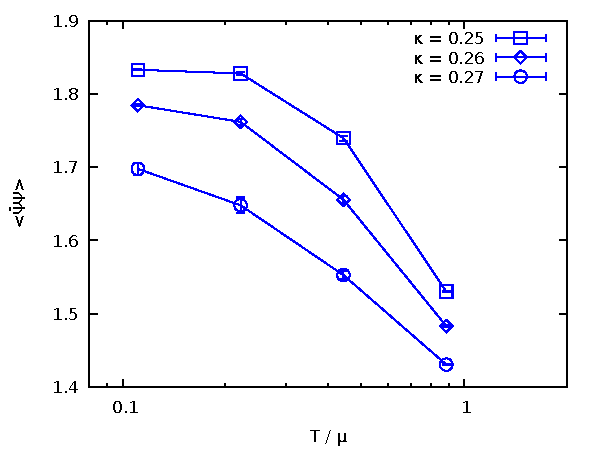
\includegraphics[width=0.8\textwidth]{Wilson/pbp-b02-mu}
  \caption{Wilson fermions, $\beta = 2$}
  \label{fig:wilson-beta2}
  \vspace{1.5cm}
  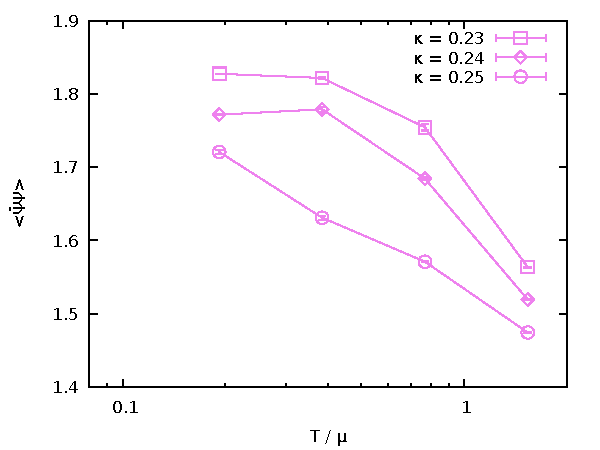
\includegraphics[width=0.8\textwidth]{Wilson/pbp-b06-mu}
  \caption{Wilson fermions, $\beta = 6$}
  \label{fig:wilson-beta6}
\end{figure}

\begin{figure}[t]
  \centering
  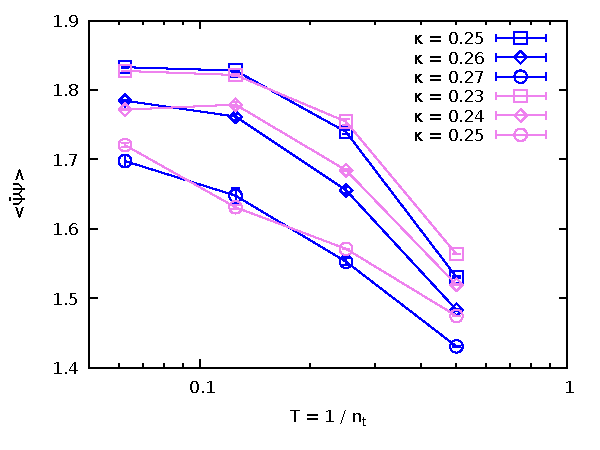
\includegraphics[width=0.8\textwidth]{Wilson/pbp-all}
  \caption{Wilson fermions, $\beta = 2$ (blue) and $\beta = 6$ (violet)}
  \label{fig:wilson-all-beta}
\end{figure}

\bibliographystyle{alpha}
\bibliography{../ref/ref}{}

\end{document}
